\begin{frame}
    \frametitle{Sensor Ultrasónico}
    \scriptsize
    
    \begin{center}
        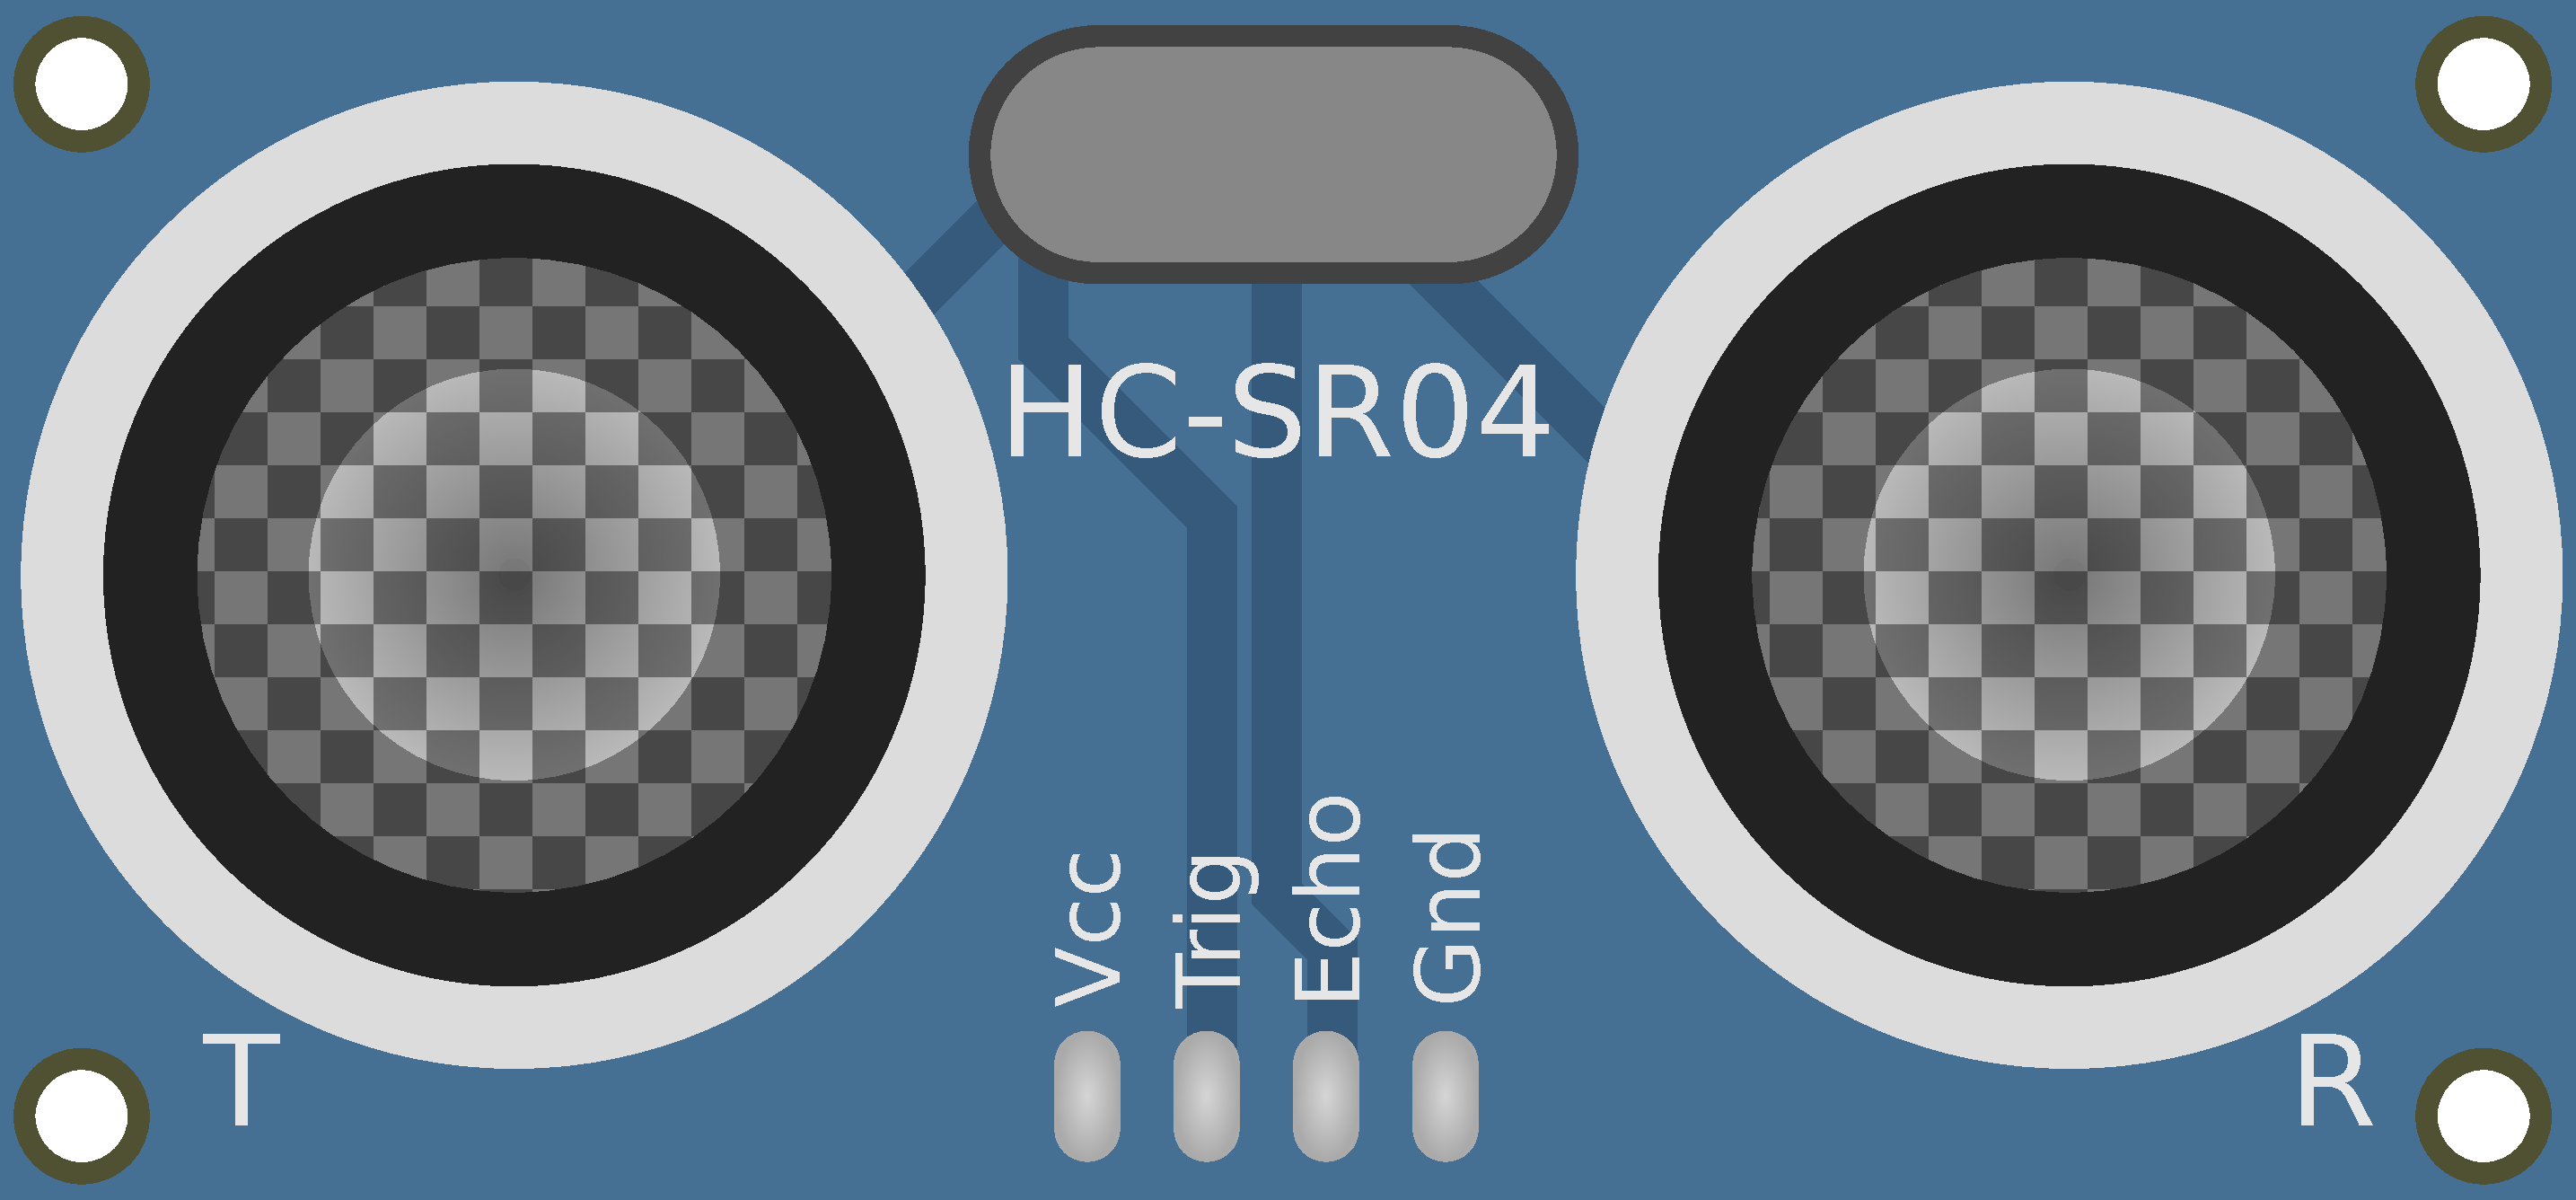
\includegraphics[width=0.2\columnwidth]{images/ultrasonic_sensor.pdf}
    \end{center}
    
    
    \begin{block}{Principio de funcionamiento}
        El principio básico de un sensor ultrasónico es transmitir un paquete de ondas de presión (ultrasónicas) y medir el tiempo que tarda este paquete de ondas en reflejarse y regresar al receptor. La distancia del objeto que causa el reflejo  $d$ se puede calcular en función de la velocidad de propagación del sonido $c$ y el tiempo de vuelo $t$.
   
        \begin{equation*}
            d = \dfrac{c t}{2}
        \end{equation*}
        La velocidad del sonido está dada por
        \begin{equation*}
            c = \sqrt{\gamma R T}
        \end{equation*}
        donde
        \begin{itemize}
            \item $\gamma$ es el ratio de calores específicos\\
            \item $R$ es la constante del gas\\
            \item $T$ es la temperatura del ambiente en grados Kelvin
        \end{itemize}
            
        En aire a presión estándar y $\SI{20}{\degree}$ la velocidad del sonido es aproximadamente $c = \SI{343}{\meter\over\second}$.
    \end{block}
\end{frame}